% !TEX root = main.tex
\section {Vergleich reaktive \& imperative Anwendung}
\label{section:vergleich_reaktiv_imperativ}
Um zu prüfen, ob Leistungsfähigkeit und Skalierbarkeit einer reaktiven Anwendung tatsächlich die einer traditionellen, imperativen Anwendung
übertrifft, werden in diesem Kapitel beide Ansätze hinsichtlich verschiedener Metriken in einem festen Zeitintervall miteinander verglichen.

\subsection{Implementierung \& Systemaufbau}
\label{section:implementierung}
Die beiden Anwendungen implementieren mit dem Quarkus-Framework jeweils eine simple REST-Schnittstelle mit HTTP-CRUD Methoden
und einer angebundenen PostgreSQL-Datenbank.
Dabei ist vorallem die HTTP-Schicht von Interesse. Die HTTP-Unterstützung von Quarkus basiert auf einem reaktiven, nicht-blockierenden
Unterbau: der Vert.x Engine.
Jede HTTP-Anfrage wird auf einem der \textit{event-loop threads} bzw. \textit{IO threads}
\footnote{Deren Anzahl hängt von der Anzahl der CPU-Kerne ab}
verarbeitet und durch eine Routing-Schicht an den Anwendungscode weitergeleitet.
Je nachdem welcher Ansatz zur Implementierung des jeweiligen HTTP-Endpunktes gewählt wurde,
wird der Code dann auf einem blockierenden \textit{worker thread} (Servlet, JAX-RS) oder einem der
\textit{IO threads} (Reactive Routes, Reactive Resteasy) ausgeführt.
Die \textit{IO threads} sind dafür zuständig alle IO-Operationen asynchron auszuführen und die jeweiligen EventListener bzw. Subscriber auszulösen sobald
die Operationen abgeschlossen sind.
\newpage
\begin{figure}[h!]
    \centering
    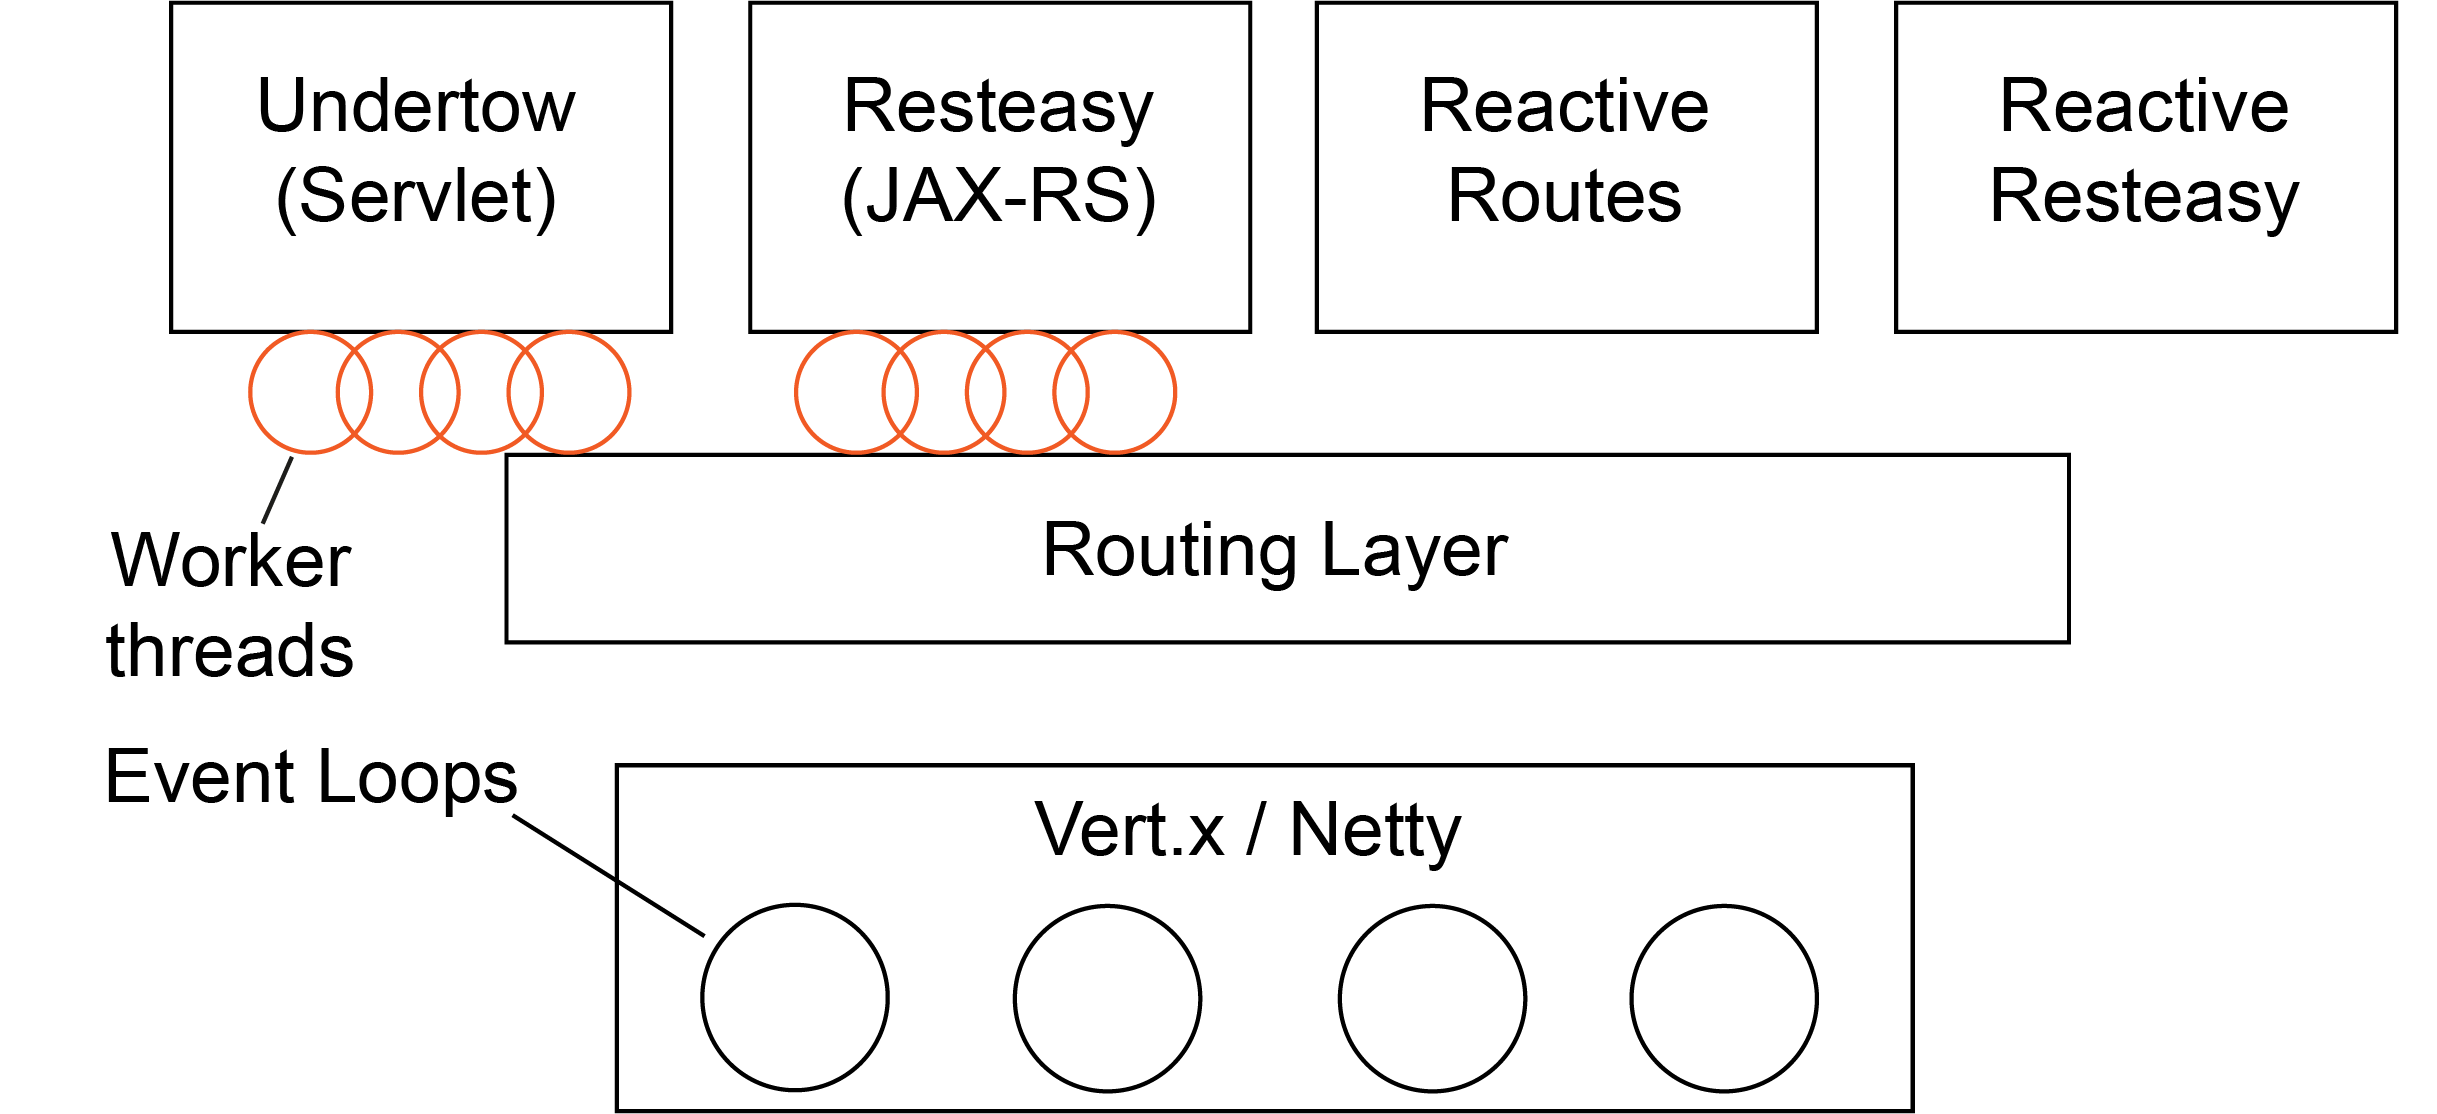
\includegraphics[width=1.0\textwidth]{Quarkus_HTTP_Layer}
    \caption{Quarkus HTTP-Schicht \parencite{QuarkusReactiveRoutes}}
\end{figure}

Damit sich beide Anwendungen nahe an einer realen Java-EE REST-API orientieren, haben
sie (zusätzlich zu den grundlegenden Abhängigkeiten des Quarkus-Frameworks) folgende Projekt-Abhängigkeiten:
\begin{enumerate}
    \item JAX-RS Implementierung
    \item JSON Unterstützung
    \item Datenbanktreiber
    \item JPA Implementierung
\end{enumerate}

Diese Abhängigkeiten wurden vom Quarkus Maven-Repository sowohl in blockierender,
als auch in nicht-blockierender, reaktiver Form bereitgestellt: \parencite{MavenQuarkusIO}
% space between the text and the left/right border of its containing cell is set to 18 pt
\setlength{\tabcolsep}{18pt}
% the height of each row is set to 1.5 relative to its default height
\renewcommand{\arraystretch}{1.5}
\begin{table}[h!]
    \centering
    \begin{tabular}{| c | c | c |}
        \hline
                         & Blockierend      & Nicht-blockierend (reaktiv) \\
        \hline
        JAX-RS           & Resteasy         & Resteasy Reactive           \\
        \hline
        JSON             & Resteasy-Jackson & Resteasy-Reactive-Jackson   \\
        \hline
        Datenbanktreiber & JDBC-Postgresql  & Reactive-Pg-Client          \\
        \hline
        JPA-/ORM         & Hibernate-ORM    & Hibernate-Reactive          \\
        \hline
    \end{tabular}
    \caption{Tabelle mit den verwendeten Anwendungen beider Applikationen}
    \label{table:dependencies}
\end{table}
Der Projekt-Code dieser Arbeit kann vom Gitlab-Server der Ostfalia unter
\url{//TODO Ostfalia Gitlab link?} eingesehen und abgerufen werden.

\subsection{Testbedingungen}
\label{section:testbedingungen}
//TODO: Erklären welche Hardware Specs und Software Versionn nötig sind, Dinge wie SSH Zugriff

\subsection{Vorgehen des Tests / Testaufbau}
\label{section:vorgehen}
//TODO: Erklären wie das gesamte System getestet wird, welche Werkzeuge (wrk2 (warum wrk2, latenzmessung im gegensatz zu wrk), top, jbang etc.
docker für reproduzierbare umgebung, lua histogramme dann durch javascript-script zu graphen )
Systemaufbau (Client-Host, Server-Host, User-Host)
//eine minute lang http anfragen an zwei Anwendungen, die genau dasselbe machen
was genau gemessen wird (welche Metriken) und wie
diees beeeinflusst werden können
Jeden größeren Schritt erklären, Bauen der Anwendungen, Warm-Up (JIT), Workload

\subsection{Test: Statische Daten}
\label{section:statische_daten}

\subsubsection{Systemablauf}
//TODO: Grafik ähnlich zu Grafik in Implementierung aber mit Threadwechseln und exemplarisch mhrere Threads zeigen
(auch angeben wie Ergebnisse mit komplizierteren Queries aussehen könnten)
\subsubsection{Resultate}

\subsection{Test: Datenbankzugriffe}
\label{section:datenbankzugriffe}

\subsubsection{Systemablauf}
//TODO: Grafik ähnlich zu Grafik in Implementierung aber ohne Threadwechsel dafür Main-Thread mit dahinterliegender Datenbank,
das Nicht BLockieren bzw. Asynchronität verdeutlichen

\subsubsection{Resultate}

\subsection{Auswertung}
\label{section:auswertung}